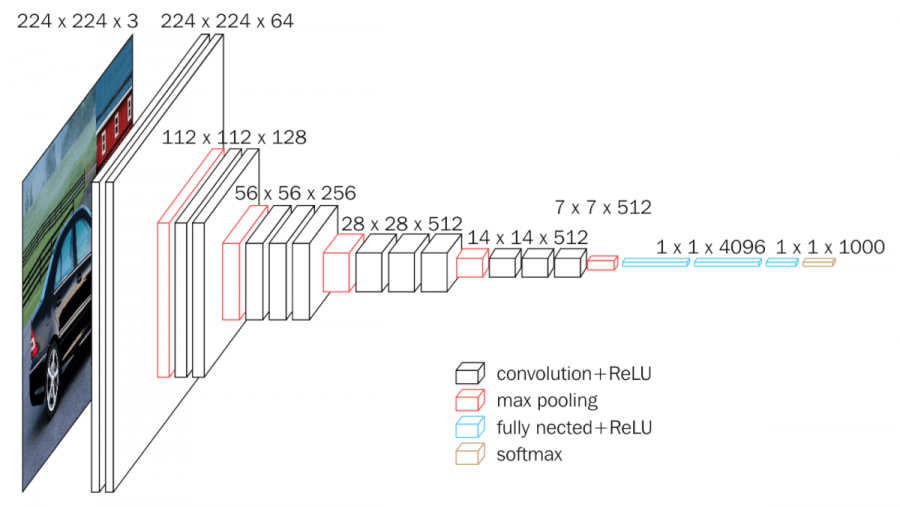
\includegraphics[scale=0.5]{images/modelOne/vgg16.png}
VGG16 is a convolutional neural network model proposed by K. Simonyan and A. Zisserman from the University of Oxford for ILSVRC-2014 competition. This model achieves 92.7% top-5 test accuracy on ImageNet dataset which contains 14 million images belonging to 1000 classes.\\
It is considered to be one of the excellent vision model architecture till date. Most unique thing about VGG16 is that instead of having a large number of hyper-parameter they focused on having convolution layers of very small receptive fields - 3x3 filter with a stride 1. It also always uses same padding and maxpool layers of 2x2 filters of stride 2. It follows this arrangement of convolution and max pool layers consistently throughout the whole architecture. In the end it have three Fully-Connected (FC) layers: the first two have 4096 channels each, the third performs 1000-way ILSVRC classification and thus contains 1000 channels (one for each class). The final layer is the soft-max layer. \\
All hidden layers are equipped with the rectification (ReLU) non-linearity. It is also noted that none of the networks (except for one) contain Local Response Normalisation (LRN), such normalization does not improve the performance on the ILSVRC dataset, but leads to increased memory consumption and computation time.\\
The 16 in VGG16 refers to it has 16 layers that have weights. This network is a pretty large network and it has about 138 million parameters.
